\documentclass[11pt,a4j,fleqn]{jarticle}
\usepackage{amsmath,amsthm,amssymb}
\usepackage[dvipdfmx]{graphicx}

\title{包絡線定理}
\author{三ツ國 拓真}
\date{2014/6/6}


\begin{document}

\maketitle

\section{包絡線定理}

包絡線とは、曲線群があるとき、その縁がなぞる曲線をいう。
一般的に曲線群と書いたが、直線群の包絡線も存在する。ここでは、直線群の包絡線について説明する。関数$f(x, t) = x t - x^2 $はxをパラメーターと見なすと、縦軸f(t)横軸tのグラフにおいて、傾きx、切片$- x^2$の直線となる。このとき、xの値を変えることによっていくつもの直線が引かれる。このグラフが図1・図2。f(x, t)はxについて二次関数なので平方完成することで$f(x, t) = -\left(x - \frac{t}{2}\right)^2 + \frac{t^2}{4} \label{eq:square-2}$が得られ、fは$x=t/2$で最大値$t^2/4$をとることから、包絡線の関数は$F=t^2/4$となる。




\begin{figure}
 \centering
 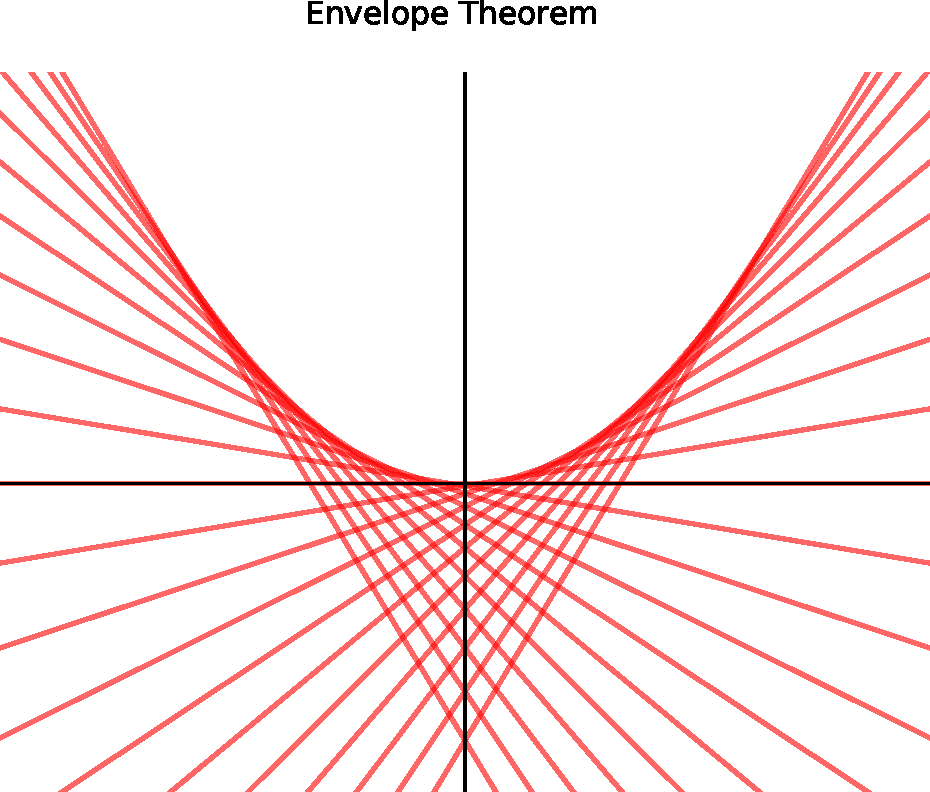
\includegraphics{envelope0.pdf}
 \caption{包絡線1}
 \label{fig:1}
\end{figure}

\begin{figure}
 \centering
 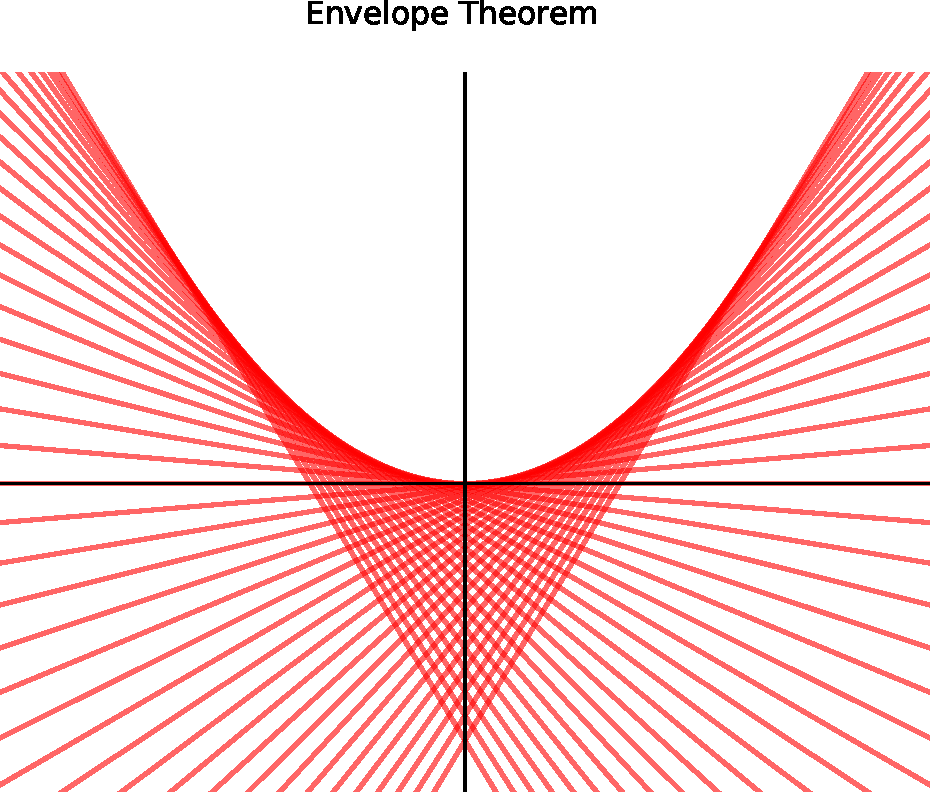
\includegraphics{envelope1.pdf}
 \caption{包絡線2}
 \label{fig:2}
\end{figure}










\section{Pythonプログラム}

\begin{quote}
\begin{verbatim}
import matplotlib.pyplot as plt
import numpy as np
import pylab as pl 
def f(x,t):     
   return t * x - t**2 #包絡線のもとの関数を定義

FIGNUM = 1 #2つのグラフを作るためにifを用いる
if FIGNUM == 0:       
    a, b, c = 0.5, -10, 11#aは~刻み、b,cはnループの範囲と包絡線の本数
if FIGNUM == 1:
    a, b, c = 0.25, -20, 21


u = a

def subplots():
    "Custom subplots with axes throught the origin"
    fig, ax = plt.subplots()

    # Set the axes through the origin
    for spine in ['left', 'bottom']:
        ax.spines[spine].set_position('zero')
    for spine in ['right', 'top']:
        ax.spines[spine].set_color('none')
    
    return fig, ax


fig, ax = subplots()  # Call the local version, not plt.subplots()
x = np.linspace(-15, 15, 100) #xの範囲設定
plt.xlim([x.min(),x.max()])  #x軸の範囲
plt.ylim([-30,40])       #y軸の範囲
ax.set_xticks([])        #x,y軸の目盛消し
ax.set_yticks([])
fig.suptitle('Envelope Theorem', fontsize=15)
for  n in range(b, c): #b~cの範囲でまわす
    y = f(x,t = n * u) #u=0.1のときはtは0.1刻みになる
    ax.plot(x, y, 'r-', linewidth=2, label='sine function', alpha=0.6)

plt.savefig('envelope' + str(FIGNUM) +  '.pdf', bbox_inches='tight', pad_inches=0)
plt.show()
\end{verbatim}
\end{quote}

正直なところ包絡線のグラフをsampleのコードからその意味を理解しながら作成するので手一杯になって工夫する余裕がなかった。Quantitative Economicsのexcerciseでもそうだが、答えや方針を与えられて理解することはなんとかできても、自身で方針や代替案を考えることのできるレベルに至っていないように思われる。慣れの問題もあると思われるので、ゼミの時間や課題以外にも自主練習を行っていきたい思う。まずは、短期費用曲線と長期費用曲線のグラフを描きたいと思う。



\begin{thebibliography}{0}
\bibitem{OyamaYasuda11}
尾山大輔・安田洋祐「経済学で出る包絡線定理」『経済セミナー』2011年10・11月号.
\end{thebibliography}

\end{document}